\section{Group Actions}
It is often easier to understand a group if it's doing something, permuting elements, rotating a square etc.

\begin{definition}[Group action]
    Let $G$ be a group and $X$ a non-empty set.
    We say that $G$ \emph{acts} on $X$ if there is a mapping
    \begin{align*}
        \rho : G \times X &\to X \\
        (g, x) &\mapsto \rho(g, x) = g(x)
    \end{align*} 
    such that 
    \begin{enumerate} \addtocounter{enumi}{-1}
        \item if $g \in G$, $x \in X$, then $\rho(g, x) = g(x) \in X$ (implied by notation, but something we should check).
        \item $\rho(gh, x) = \rho(g, \rho(h, x))$. shorthand: $gh(x) = g(h(x))$. \label{action-1}
        \item $\rho(e, x) = x$, shorthand: $e(x) = x$.
    \end{enumerate} 
    When $G$ acts on a set it maps elements of $X$ to $X$ in a way that the multiplication of $G$ is respected.
\end{definition} 

\begin{example} \label{exm:actions} \mbox{}
    \begin{enumerate} \def\labelenumi{\roman{enumi}.} \def\labelenumii{\arabic{enumii}.} 
        \item trivial action $\rho(g, x) = x \; \forall \; x \in X, g \in G$.
        \item $S_n$ acts on $X = \{ 1, 2, \ldots, n \}$ by permuting the elements of $X$.
        e.g. $S_3$ acts on $\{1, 2, 3\}$, $\sigma = \begin{pmatrix}1 & 2\end{pmatrix} \in S_3 : \sigma(1) = 2, \sigma(2) = 1, \sigma(3) = 3$.
        $\tau = \begin{pmatrix}1 & 3\end{pmatrix} \in S_3$, $\tau \sigma = \begin{pmatrix}1 & 3\end{pmatrix} \begin{pmatrix}1 & 2\end{pmatrix} = \begin{pmatrix}1 & 2 & 3\end{pmatrix}$ \\
        $(\tau \sigma)(1) = 2$, $\tau(\sigma(1)) = \tau(2) = 3$. \\
        Similarly subgroups of $S_n$ act on $X$.
        \item $D_8 = \{e, r, r^2, r^3, t, rt, r^2t, r^3t \}$ acts on the edges of a square.
        \begin{figure}
            \centering 
            \includegraphics[height=5cm]{figures/06-square-action}
        \end{figure} 
        \begin{align*}
            t(a) &= c & t(c) &= a \\
            t(b) &= b & t(d) &= d. \\
            r(a) &= b.
        \end{align*} 
        Also acts on the vertices of a square.
        \begin{figure}
            \centering 
            \includegraphics[height=5cm]{figures/06-square-action-vertex}
        \end{figure} 
        \begin{align*}
            t(1) &= 4 & t(4) &= 1 \\
            t(2) &= 3 & t(d) &= 2.
        \end{align*} 
        \item $G$ acts on itself by left multiplication.
        This is called the \emph{left regular action}
        \begin{align*}
            G \times G &\to G \\
            (g, k) &\mapsto gk.
        \end{align*} 
        Check:
        \begin{enumerate} \addtocounter{enumii}{-1}
            \item $gk \in G$ (by closure)
            \item
            \begin{align*}
                \rho(gh, k) &= ghk \\
                \rho(g, \rho(h, k)) &= \rho(g, hk) = ghk \\
                \intertext{Or in shorthand: }
                gh(k) &= ghk \\
                g(h(k)) &= g(hk) = ghk.
            \end{align*} 
            \item $\rho(e, k) = ek = k$.
        \end{enumerate} 
        \item We also have the $G$ \emph{right regular action}
        \begin{align*}
            G \times G &\to G \\
            (g, k) &\mapsto k g^{-1}.
        \end{align*} (we need inverse for \Cref{action-1} to hold.)
        \item $G$ acts on itself by \emph{conjugation}
        \begin{align*}
            G \times G &\to G \\
            (g, k) &\mapsto gkg^{-1}.
        \end{align*} 
        Check: 
        \begin{enumerate} \addtocounter{enumii}{-1}
            \item $gkg^{-1} \in G$ (by closure)
            \item
            \begin{align*}
                \rho(gh, k) &= ghk(gh)^{-1} \\
                &= gh k h^{-1} g^{-1}
                \rho(g, \rho(h, k)) &= \rho(g, hkh^{-1}) = g (h k h^{-1}) g^{-1}
            \end{align*} 
            \item $\rho(e, k) = ek e^{-1} = k$.
        \end{enumerate} 
        \item Let $N \trianglelefteq G$, then $G$ acts on $N$ by conjugation
        \begin{align*}
            G \times N &\to N \\
            (g, n) &\mapsto gng^{-1}.
        \end{align*} 
        0.  $gng^{-1} \in G$ since $N \trianglelefteq G$. \\
        (1) and (2) as above.
        \item Let $H \leq G$, then $G$ acts on the set of left cosets, $(G : H)$, if $H$ in $G$.
        Called the \emph{left coset action}.
        \begin{align*}
            G \times (G : H) &\to (G : H) \\
            (g, kH) &\mapsto gkH.
        \end{align*} 
        \begin{enumerate} \addtocounter{enumii}{-1}
            \item $gkH \in (G : H)$
            \item
            \begin{align*}
                \rho(gh, kH) &= (gh)kH = gh kH. \\
                \rho(g, \rho(h, kH)) &= \rho(g, hkH) \\
                &= g h k H
            \end{align*} 
            \item $\rho(e, kH) = ek H = kH$.
        \end{enumerate} 
    \end{enumerate} 
\end{example} 

\begin{remark}
    Recall a permutation of a set $X$ is a bijection of $X$, \Cref{def:permutation}.
    We have commented that a bijection $f : X \to X$ has a 2-sided inverse, i.e. $\exists \; g : X \to X$ s.t.
    \begin{align*}
        f \circ g (x) &= x \; \forall \; x \in X \\
        g \circ f (x) &= x \; \forall \; x \in X.
    \end{align*}
    Conversely if $f : X \to X$ is a map with a 2-sided inverse then $f$ is a bijection.

    $f \circ g(x) = x \; \forall \; x \in X \implies f$ is surjective, as $f$ is mapping to all elements in $X$ \\
    $g \circ f(x) = x \; \forall \; x \in X \implies f$ is injective, as if $f$ took two elements to the same place then $g$ wouldn't be able to split them up.

    Note 2-sided is necessary:
    \begin{align*}
        \phi : \mathbb{Z} &\to \mathbb{Z} & \psi : \mathbb{Z} &\to \mathbb{Z}\\
        x &\mapsto 2x & 2x & \mapsto x \\
        && 2x + 1 &\mapsto 0 \\
        \phi \psi &= \operatorname{id}. &&
    \end{align*} 
\end{remark} 

\begin{lemma} \label{lem:16}
    Suppose the group $G$ acts on the non-empty set $X$.
    Fix $g \in G$, then the 
    \begin{align*}
        \phi_g : X &\to X \\
        x &\mapsto \rho(g, x) = g(x)
    \end{align*} is a permutation of $X$, i.e. $\phi_g = \operatorname{Sym}(X)$.
\end{lemma} 

\begin{proof}
    Clearly $\phi_g$ is a map from $X$ to $X$.
    We need to show $\phi_g$ is a bijection, enough to show it has a 2-sided inverse.
    %
    \begin{align*}
        \phi_{g^{-1}} \circ \phi_g (x) &= \phi_{g^{-1}} \left( \rho (g, x) \right) \\
        &= \rho(g^{-1}, \rho(g, x)) \\
        &= \rho(g^{-1} g, x) \text{ since $\rho$ is a group action, \ref{action-1}} \\
        &= \rho(e, x) \\
        &= x \; \forall \; x.
    \end{align*} 
    Similarly, $\phi_g \circ \phi_{g^{-1}}(x) = x \; \forall \; x \in X$.
\end{proof} 

\begin{proposition} \label{prp:6}
    Suppose $G$ acts on the set $X$.
    Then the map 
    \begin{align*}
        \Phi : G &\to \operatorname{Sym}(x) \\
        g &\mapsto \phi_g
    \end{align*} as in \Cref{lem:16}, is a homomorphism.
\end{proposition}  

\begin{proof}
    We need to show $\Phi$ is a homomorphism i.e. need
    \begin{align*}
        \Phi(gh) &= \Phi(g) \circ \Phi(h) \\
        \text{i.e. } \phi_{gh} &= \phi_g \circ \phi_h.
    \end{align*}  
    Let $x \in X$
    \begin{align*}
        \phi_{gh}(x) &= \rho(gh, x) \\
        &= \rho(g, \rho(h, x)) \\
        &= \phi_g \circ \phi_h (x).
    \end{align*} 
    This is true $\forall \; x \in X$.
\end{proof} 

\begin{remark} \mbox{}
    \begin{enumerate} \def\labelenumii{\roman{enumii}.} 
        \item \Cref{prp:6} gives us an equivalent definition of a group action.
        If $G$ is a group and $X$ a set such that $\Phi: G \to \operatorname{Sym}(X)$ is a group homomorphism, then 
        \begin{align*}
            \rho : G \times X &\to X \\
            (g, x) &\mapsto \phi_g(x)
        \end{align*} where $\Phi(g) = \phi_g$, is group action.
        \item Using notation of \Cref{prp:6}, by \nameref{thm:six} 
        \begin{align*}
            G / \ker \Phi &\cong \operatorname{Im} \Phi \leq \operatorname{Sym}(X).
            \intertext{Note}
            \ker \Phi &= \{g \in G : \Phi(g) = \text{id}_X \in \operatorname{Sym}(X) \\
            &= \{ g \in G : \phi_g(x) = \rho(g, x) = x \ \forall \; x \in X \} \\
            &\trianglelefteq G \text{ Kernels of homomorphisms are normal subgroups (Sheet 1, q9)}. 
        \end{align*} 
        I.e. all those elements that fix every elements of $X$, that act 'trivially'.

        We say the action is \emph{faithful} if $\ker \Phi = \{ e \}$.

        e.g. the kernels of \Cref{exm:actions}
        \begin{enumerate}
            \item trivial action - $\ker \Phi = G$.
            \item $S_n$ acts on $\{1, \ldots, n\}$ - faithful.
            \item $D_8$ acts on the edges of a square - faithful.
            \item left regular action - faithful.
            \item conjugation - $\ker \Phi = \{g \in G : \underbrace{g k g^{-1} = k}_{gk = kg} \ \forall \; k \in G\} = Z(G)$, the \emph{the centre of} $G$. 'the elements that commute with everything'.
            \item conjugation of $N \trianglelefteq G$. $\ker \Phi = \{ g \in g : g n g^{-1} = n \ \forall \; n \in N\} = C_G(N)$, the \emph{centraliser of $N$ in $G$}.
            \item left coset action -
            \begin{align*}
                \ker \Phi &= \{ g \in G: g kH = kH \ \forall \; k \in G\} \\
                &= \{ g \in G: k^{-1}gk \in H \ \forall \; k \in G\} \\
                &= \{g \in G : g \in k H k^{-1} \ \forall \; k \in G\} \\
                &= \bigcap_{k \in G} k H k^{-1}  \\
                &= \operatorname{Core}_G(H) \trianglelefteq G \\
                \text{and } \underbrace{\operatorname{Core}_G(H)}_\text{core of $H$} &\leq H \text{ (we can set $k = e$)}.
            \end{align*} 
            \emph{Useful Note for exm sheet:} If $\ker \Phi = \{ e \}$, then $G$ is isomorphic to a subgroup of $\operatorname{Sym}(X)$, we write $G \lesssim \operatorname{Sym}(X)$.
            So if $|G| \nmid |\operatorname{Sym}(X)|$ then $\ker \Phi \neq \{e\}$.
        \end{enumerate} 
    \end{enumerate} 
\end{remark} 

\begin{theorem}[Cayley's Theorem] \label{thm:7}
    Any group $G$ is isomorphic to a subgroup of $\operatorname{Sym}(X)$ for some non-empty set $X$.
\end{theorem} 

\begin{proof}
    We take $X$ to be $G$ and consider the left regular action
    \begin{align*}
        G \times G &\to G \\
        (g, h) &\mapsto gh.
    \end{align*} 
    This is a faithful action as $gh = h \; \forall \; h \in G \implies g = e$.
    Thus we have an injective homomorphism 
    \begin{align*}
        \Phi : G &\to \operatorname{Sym}(G)
    \end{align*} and $G \lesssim \operatorname{Sym}(G)$.
\end{proof} 

\begin{definition}[Orbit] \label{def:17}
    Let $G$ act on a set $X$ and $x \in X$.
    The \emph{orbit} of $x \in X$ is given by 
    \begin{align*}
        \operatorname{Orb}_G (x) = \{g(x) : g \in G \} \subseteq X.
    \end{align*} 
    I.e. the set of points in $X$ which $x$ can be mapped to.
\end{definition} 

\begin{example} \mbox{}
    The orbits of \Cref{exm:actions}.
    \begin{enumerate}
        \item trivial action, $\operatorname{Orb}_G (x) = \{ x \}$
        \item $S_n$ acts on $\{1, \ldots, n\}$ - $\operatorname{Orb}_G(1) = X$ (we can get $(1\ a)$ which maps $x$ to any $a$). \\
        If $H = \langle (1\ 2) (3\ 4\ 5) \rangle \leq S_n$ acting on $X = \{ 1, 2, 3, 4, 5\}$ then $\operatorname{Orb}_G(1) = \{1, 2\}$ and $\operatorname{Orb}_G(3) = \{3, 4, 5\}$.
        \item $D_8$ acts on the edges of a square - $\operatorname{Orb}_{D_8}(a) = \{a, b, c, d\}$.
        \item left regular action - $\operatorname{Orb}_G(k) = G$, since $g = g(k^{-1}k) = (gk^{-1})k$ for any $g \in G$.
        \item conjugation - $\operatorname{Orb}_G(k)$
        \begin{align*}
            \operatorname{Orb}_G(k) &= \{g(k) : g \in G\} \\
            &= \{ gkg^{-1} : g \in G \} \\
            &= \operatorname{ccl}_G(k)
        \end{align*}, the \emph{conjugacy class of $k$ in $G$}. If $h \in \operatorname{ccl}_G(k)$ we say $h$ and $k$ are \emph{conjugate}.
    \end{enumerate} 
\end{example} 

\begin{definition}[Transitive orbits] \label{def:18}
    We say $G$ acts \emph{transitively} on $X$ if for any $x \in X$, $\operatorname{Orb}_G(x) = X$.
    Equivalently, if given any pair $x_1, x_2 \in X \; \exists \; g \in G$ s.t. $g(x_1) = x_2$.

    So the left regular action is a transitive action.
\end{definition} 

\begin{lemma} \label{lem:17}
    The distinct $G$-orbits form a partition of $X$
\end{lemma} 

\begin{proof}
    Let $x \in X$, then $x \in \operatorname{Orb}_G(x)$ since $x = ex$. \\
    Suppose $z \in \operatorname{Orb}_G(x) \cap \operatorname{Orb}_G(y)$, we show $\operatorname{Orb}_G(x) = \operatorname{Orb}_G(z) = \operatorname{Orb}_G(y)$. \\
    $z \in \operatorname{Orb}_G(x) \implies \exists \; g \in G$ s.t. $g(x) = z$.
    \begin{align*}
        \text{Suppose } t \in \operatorname{Orb}_G(z) \implies \exists \; h &\in G \text{ s.t. } h(z) = t \\
        \implies t &= h(g(x)) = (hg)(x) \\
        \implies t &\in \operatorname{Orb}_G(x)
        \implies \operatorname{Orb}_G(z) \subseteq \operatorname{Orb}_G(x)
        \text{Similarly } g(x) &= z \\
        x &= e(x) = (g^{-1} g)(x) = g^{-1}(z) \\
        \implies \operatorname{Orb}_G(x) \subseteq \operatorname{Orb}_G(z).
    \end{align*} 
    Thus $\operatorname{Orb}_G(x) = \operatorname{Orb}_G(z)$.
    Similarly, $\operatorname{Orb}_G(z) = \operatorname{Orb}_G(y)$.
\end{proof} 

\begin{remark} \mbox{}
    \begin{enumerate}
        \item We could have proved \Cref{lem:17} by noticing that $x_1 \sim x_2$ if $\exists \; g \in G$ s.t. $g(x_1) = x_2$ is an equivalence relation.
        \item $\operatorname{Orb}_G(x)$ is $G$-invariant, i.e. $g \left( \operatorname{Orb}_G(x) \right) \subseteq \operatorname{Orb}_G(x)$.
        Since if $y \in \operatorname{Orb}_G(x), y = hx$ for some $h \in G \implies g(y) = g(h(x)) = (gh)(x) \in \operatorname{Orb}_G(x)$.
        \item $G$ is transitive on $\operatorname{Orb}_G(x)$.
        \begin{align*}
            \text{Let } y, z &\in \operatorname{Orb}_G(x) \\
            y &= g(x), z = h(x), \text{ for some } g, h \in G. \\
            \text{Then } z &= h(g^{-1}(y)).
        \end{align*} 
    \end{enumerate} 
\end{remark} 

\begin{definition}[Stabiliser] \label{def:19}
    Let $G$ act on $X$ and $x \in X$.
    The \emph{stabiliser} of $x$ in $G$ is given by
    \begin{align*}
        \operatorname{Stab}_G(x) &= \{ g \in G : g(x) = x \} \\
        &\subseteq G.
    \end{align*} 
    i.e. all those elements in $G$ that fix $x$.
\end{definition} 

\begin{example} \mbox{}
    The stabilisers of \Cref{exm:actions}.
    \begin{enumerate}
        \item trivial action - $\operatorname{Stab}_G(x) = G$.
        \item $S_n$ on $X = \{1, 2, \ldots, n\}$ - $\operatorname{Stab}_G(1) \cong S_{n-1}$.
        \item $H = \langle \begin{pmatrix}1 & 2\end{pmatrix} \begin{pmatrix}3 & 4 & 5\end{pmatrix} \rangle$ on $X$ - $\operatorname{Stab}_H(1) = \langle \begin{pmatrix}3 & 4 & 5\end{pmatrix} \rangle$.
        \item $D_8$ - $\operatorname{Stab}_{D_8}(b) = \{e, t\}$. \\
        \item left regular action - $\operatorname{Stab}_G(k) = \{e\}$, $gk = k \implies g = e$.
        \item conjugation - \begin{align*}
            \operatorname{Stab}_G(k) &= \{g \in G : g(k) = k\} \\
            &= \{g \in G : g k g^{-1} = k\} \\
            &= \{g \in G : g k = kg \} \\
            &= C_G(k), \emph{ centraliser of $k$ in $G$}.
        \end{align*} I.e. all those elements of $G$ that commute with $k$.
    \end{enumerate} 
\end{example} 

\begin{lemma} \label{lem:18}
    $\operatorname{Stab}_G(x)$ is a subgroup of $G$.
\end{lemma} 

\begin{proof} \mbox{}
    \begin{itemize} 
        \item $e(x) = x \implies e \in \operatorname{Stab}_G(x)$.
        \item \begin{align*}
            \text{if } g, h &\in \operatorname{Stab}_G(x) \\
            (gh)(x) &= g(h(x)) \\
            &= g(x) \\
            &= x \implies gh \in \operatorname{Stab}_G(x).
            \end{align*} 
        \item \begin{align*}
            g &\in \operatorname{Stab}_G(x) \\
            g(x) &= x \\
            x &= e(x) = (g^{-1} g)(x) = g^{-1}(gx) \\
            &= g^{-1}(x) \\
            \implies g^{-1} &\in \operatorname{Stab}_G(x).
        \end{align*} 
        \item Associativity is inherited from $G$.
    \end{itemize} 
\end{proof} 

\begin{remark} 
    Recall, \Cref{prp:6} \begin{align*}
        \Phi : G &\to \operatorname{Sym}(X) \\
        \ker \Phi &= \{ g \in G : g(x) = x \; \forall \; x \in X \} \\
        &= \bigcap \operatorname{Stab}_G(x).
    \end{align*}
\end{remark} 

\begin{theorem}[Orbit-Stabiliser Theorem] \label{thm:orbit}
    Let $G$ be a finite group acting on a non-empty set $X$.
    Then $\operatorname{Stab}_G(x) \leq G$ and 
    \begin{align*}
        |G| = |\operatorname{Stab}_G(x)| |\operatorname{Orb}_G(x)|.
    \end{align*} 
\end{theorem} 

\begin{remark}
    We actually prove that $|G : \operatorname{Stab}_G(x)|$, the number of left cosets of $\operatorname{Stab}_G(x)$ in $G$, is equal to $|\operatorname{Orb}_G(x)|$, a more general statement.
\end{remark} 

\begin{proof}
    $(G : \operatorname{Stab}_G(x))$ is the set of left cosets of $\operatorname{Stab}_G(x)$ in $G$.
    Consider the map 
    \begin{align*}
        \theta : \operatorname{Orb}_G(x) &\to (G : \operatorname{Stab}_G(x)) \\
        g(x) &\mapsto g \operatorname{Stab}_G(x).
    \end{align*}  
    $\theta$ is well-defined: 
    \begin{align*}
        g(x) = h(x) \implies h^{-1}g(x) (x) &= x \\
        \implies h^{-1}g &\in \operatorname{Stab}_G(x) \\
        \implies g \operatorname{Stab}_G(x) &= h \operatorname{Stab}_G(x) \text{ by \Cref{lem:eleven}} \\
        \implies \theta(g(x)) &= \theta(h(x)).
    \end{align*} 
    $\theta$ is injective: 
    \begin{align*}
        \theta(g(x)) &= \theta(h(x)) \\
        \implies g \operatorname{Stab}_G(x) &= h \operatorname{Stab}_G(x) \\
        \implies h^{-1}g &\in \operatorname{Stab}_G(x) \text{ by \Cref{lem:eleven}} \\
        \implies h^{-1}g(x) &= x \\
        \implies g(x) &= h(x).
    \end{align*}
    $\theta$ is surjective:
    \begin{align*}
        \text{Given } g \operatorname{Stab}_G(x) &\in (G : \operatorname{Stab}_G(x)) \\
        \text{then } g(x) &\in \operatorname{Orb}_G(x) \\
        \text{ and } \theta(g(x)) &= g \operatorname{Stab}_G(x).
    \end{align*} 
    Thus $\theta$ is a well-defined bijection.
\end{proof} 

\subsection{Application to Symmetry Groups of Regular Solids}
Let $S$ be a regular solid and $V$ its vertices.
The the symmetries of $S$ are the isometries (distance preserving maps) of $\mathbb{R}^2$ or $\mathbb{R}^3$ that maps $S$ to itself.
The dual is the solid with vertices in the middle of each face of the input.

\subsubsection{Tetrahedron (self-dual)}

\begin{figure}
    \centering 
    \includegraphics[height=5cm]{figures/07-tetrahedron}
\end{figure} faces are $4$ equilateral triangles.

Let $G$ be group of symmetries of $T$, and $X = \{\text{vertices of } T\} = \{1, 2, 3, 4\}$.
Then $\exists$ a homomorphism
\begin{align*}
    \Phi : G &\to \operatorname{Sym} X \cong S_4 \text{ \Cref{prp:6}}
\end{align*} 
Note $\ker \Phi = \{ e \}$, if all vertices are fixed, then $T$ fixed. \\
Consider $G^+ \leq G$ be the subgroup of all rotations.
The elements of $G^+$ are as follows:

\begin{figure}
    \centering 
    \includegraphics[height=5cm]{figures/07-tetrahedron-rotations} 
    \caption{Rotation of $2 \pi / 3$, a 3-cycle $\begin{pmatrix}2 & 3 & 4\end{pmatrix}$, and $4 \pi / 3$ gives $\begin{pmatrix}2 & 4 & 3\end{pmatrix}$.}
\end{figure}

There are $4$ such axes, giving $8$ rotations of order $3$ (these are all the $3$-cycles in $S_4$).

\begin{figure} 
    \centering 
    \includegraphics[height=5cm]{figures/07-tetrahedron-double-transposition} 
    \caption{Rotation of $\pi$, a double transposition $\begin{pmatrix}1 & 4\end{pmatrix} \begin{pmatrix}2 & 3\end{pmatrix}$. We have one rotation for each pair of axes and we have $6$ axes, so $3$ such double transpositions.}
\end{figure}

and identity, 
\begin{align*}
    \implies G^+ \cong A_4.
\end{align*} (only subgroup of order $12$)

Now consider $G$ (all symmetries).
Clearly $\operatorname{Orb}_G(1) = \{1, 2, 3, 4\} = \operatorname{Orb}_{G^+}(1)$. \\
Consider $\operatorname{Stab}_G(1)$.

\begin{itemize}
    \item Note if $3$ vertices are fixed then $T$ is fixed.

    \item Suppose vertices $1$ and $2$ are fixed
    \begin{figure} 
        \centering 
        \includegraphics[height=5cm]{figures/07-tetrahedron-12-fixed} 
        \caption{reflection through $1, 2$ giving $\begin{pmatrix}3 & 4\end{pmatrix} = \tau$. We have such a reflection for each of the $6$ edges.}
    \end{figure}

    \item If just $1$ is fixed we have order $3$ rotation from before, $\sigma$.
\end{itemize} 
These are all elements in $G$
\begin{align*}
    \operatorname{Stab}_G(1) &= \langle \sigma, \tau \rangle \cong D_6 \\
    \implies |G| &= |\operatorname{Orb}_G(1)| |\operatorname{Stab}_G(1)| \text{ \nameref{thm:orbit}}\\
    &= 4 \times 6 = 24 \\
    \implies G &\cong S_4.
\end{align*} (consider the effects of $\sigma$ and $\tau$ on the bottom face to see why $\langle \sigma, \tau \rangle \cong D_6$).

Note $\operatorname{Stab}_{G^+}(1) = \langle G \rangle$.
Also $\begin{pmatrix}1 & 2 & 3 & 4\end{pmatrix} = \begin{pmatrix}1 & 2\end{pmatrix} \begin{pmatrix}2 & 3 & 4\end{pmatrix}$.

\subsubsection{Cube (dual to octahedron)}

\begin{figure} 
    \centering 
    \includegraphics[height=5cm]{figures/07-cube} 
\end{figure}

Let $G^+$ be the group of rotations of $C$.
Then $G^+$ acts on set of diagonals $X = \{D_1, D_2, D_3, D_4\}$.

If a rotation, $\sigma$, that fixes all the diagonals, then $\sigma = \text{id}$.
So we have an injective homomorphism
\begin{align*}
    \Phi : G^+ &\to \operatorname{Sym}(X) \cong S_4.
\end{align*} 
Rotations: 
\begin{itemize}
    \item $\text{id}$
    \item \begin{figure} 
        \centering 
        \includegraphics[height=5cm]{figures/04-cube-rotated}
        \caption{$\sigma$ rotation of $\pi / 2$ corresponds to $\begin{pmatrix}1 & 2 & 3 & 4\end{pmatrix}$ in action on diagonals. There are $3$ such axes giving $6$ elements of order $4$ and $3$ of order $2$.}
    \end{figure}
    \item \begin{figure} 
        \centering 
        \includegraphics[height=5cm]{figures/07-cube-rotated-fixed-axis} 
        \caption{$o(\rho) = 3$ corresponds to $\begin{pmatrix}2 & 3 & 4\end{pmatrix}$, we have 4 such axes giving eight elements of order $3$ ($\rho, \rho^2$).}
    \end{figure}
    \item \begin{figure} 
        \centering 
        \includegraphics[height=5cm]{figures/07-cube-transpositions}
        \caption{rotation of $\pi$, $o(\tau) = 2$ corresponds to $\begin{pmatrix}1 & 3\end{pmatrix}$. There are 6 such axes}
    \end{figure}
\end{itemize}
I.e. $G^+ \cong S_4$.
Note $\operatorname{Orb}_{G^+}(D_1) = \{ D_1, D_2, D_3, D_4 \}$.
$\operatorname{Stab}_{G^+}(D_1) = \{\rho, \tau'\}$
or consider $G^+$ acting on vertex $1$
\begin{align*}
    |\operatorname{Orb}_{G^+}(1)| &= 8 \\
    |\operatorname{Stab}_{G^+}(1)| &= |\langle \rho \rangle| = 3. \\
    \implies |G^+| &= 24.
\end{align*} 

Now consider full symmetry group of $C$, call it $G$.

Consider action on faces $F_1, \ldots, F_6$, this yields an injective (or faithful) homomorphism as fixing all the faces fixes everything.

\begin{align*}
    \Phi: G &\to \operatorname{Sym}(F_i) \cong S_6. \\
    |\operatorname{Orb}(F_1)| &= 6. \\
    \operatorname{Stab}(F_1) &\cong D_8. \text{ Consider the opposite face} \\
    \implies |G| &= 6 \times 8 = 48.
\end{align*} 
So, action on diagonals is not faithful; $\exists \; g \in G \ g(D_i) = D_i \ 1 \leq i \leq 4$ but $g \neq \text{id}$. 
$g$ can swap vertex $i$ with $i'$, the diagonals will stay unchanged however.
Alternatively, label vertices of $C$ as $\{(\pm 1, \pm 1, \pm 1)\}$, then 
\begin{align*}
    g : (x, y, z) &\mapsto (-x, -y, -z).
\end{align*} 
If we label the faces of the cube like a dice (1 opposite 6, 2 opposite 5, 3 opposite 4) then $g = \begin{pmatrix} 1 & 6\end{pmatrix} \begin{pmatrix}2 & 5\end{pmatrix} \begin{pmatrix}3 & 4\end{pmatrix}$.

Then $G \cong G^+ \times \langle g \rangle$.
\begin{proof}
    \begin{align*}
        G^+ &\trianglelefteq G \text{ by \Cref{lem:twelve} (since of index 2)} \\
        \langle g \rangle &\trianglelefteq G \text{ commutes with all rotations} \\
        G^+ \cap \langle g \rangle &= \{ e \} \\
        | G^+ \langle g \rangle | &= 48 = |G|.
    \end{align*} 
\end{proof} 

In fact, we have also proved that the group of symmetries of an octahedron is $S_4\times C_2$ since the octahedron is the dual of the cube. (if you join the centers of each face of the cube, you get an octahedron)
\begin{center}
  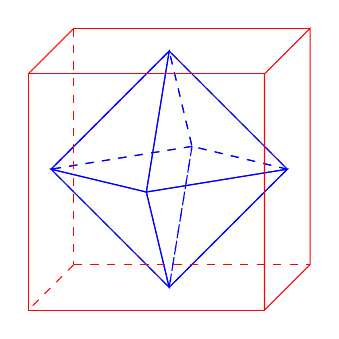
\begin{tikzpicture}[z = -5.5, scale = 1.5]
    \coordinate (O1) at (0, 0, -1);
    \coordinate (O2) at (-1, 0, 0);
    \coordinate (O3) at (0, 0, 1);
    \coordinate (O4) at (1, 0, 0);
    \coordinate (O5) at (0, 1, 0);
    \coordinate (O6) at (0, -1, 0);

    \draw [draw = blue, dashed] (O1) -- (O2) -- (O5) -- cycle;
    \draw [draw = blue, dashed] (O4) -- (O1) -- (O5) -- cycle;
    \draw [draw = blue, dashed] (O1) -- (O2) -- (O6) -- cycle;
    \draw [draw = blue, dashed] (O4) -- (O1) -- (O6) -- cycle;
    \draw [draw = blue] (O2) -- (O3) -- (O5) -- cycle;
    \draw [draw = blue] (O3) -- (O4) -- (O5) -- cycle;
    \draw [draw = blue] (O2) -- (O3) -- (O6) -- cycle;
    \draw [draw = blue] (O3) -- (O4) -- (O6) -- cycle;

    \coordinate (C1) at (-1, -1, -1);
    \coordinate (C2) at (-1, -1, 1);
    \coordinate (C3) at (-1, 1, 1);
    \coordinate (C4) at (-1, 1, -1);
    \coordinate (C5) at (1, -1, -1);
    \coordinate (C6) at (1, -1, 1);
    \coordinate (C7) at (1, 1, 1);
    \coordinate (C8) at (1, 1, -1);

    \draw [draw = red, dashed] (C1) -- (C2);
    \draw [draw = red] (C2) -- (C3);
    \draw [draw = red] (C3) -- (C4);
    \draw [draw = red, dashed] (C4) -- (C1);
    \draw [draw = red] (C5) -- (C6) -- (C7) -- (C8) -- cycle;
    \draw [draw = red, dashed] (C1) -- (C5);
    \draw [draw = red] (C2) -- (C6);
    \draw [draw = red] (C3) -- (C7);
    \draw [draw = red] (C4) -- (C8);
  \end{tikzpicture}
\end{center}

\subsubsection{Dodecahedron (dual to Icosahedron) - Non examinable}

Let $D$ be the dodecahedron.

\begin{itemize}
    \item 12 regular pentagonal faces
    \item 30 edges
    \item 20 vertices
\end{itemize} 

Let $G^+ =$ group of rotations of $D$. \\
Let $F$ be a face of $D$.
\begin{align*}
    | \operatorname{Orb}_{G^+}(F)| &= 12 \\
    | \operatorname{Stab}_{G^+}(F) | &= 5 \text{ just rotating about face} \\
    \implies |G^+| &= 5 \times 12 = 60 \text{ by \nameref{thm:orbit}.}
\end{align*} 

There are five cubes embedded in $D$.

\begin{figure}
    \centering
    \includegraphics[height=5cm]{figures/07-cube-dodecahedron}
\end{figure} 

15 pairs of edges, 3 pairs per cube $\implies$ 5 cubes.

$G^+$ acts faithfully on cubes, giving us an injective map $\Phi : G^+ \to S_5$.
And $|G^+| = 60 \implies G^+ \cong A_5$ ($A_5$ is the only subgroup of order 60 of $S_5$).
The smallest non-abelian simple group comes up as the rotational group of a dodecahedron.

We can find the elements of $A_5$
\begin{itemize}
    \item Rotations through opposite faces - 5 cycles (6 axes, 4 elements per axis giving 24 elements).
    \item Rotations through opposite vertices - 3 cycles.
    \item Rotations through opposite edges - double transpositions (15 such).
\end{itemize} 

\subsubsection{Another Application of \nameref{thm:orbit}}

\begin{theorem}[Cauchy's Theorem] \label{thm:8}
    Let $G$ be a finite group and $p$ a prime that divides $|G|$.
    Then there exists an element in $G$ of order $p$.
\end{theorem} 

\begin{proof}
    Let
    \begin{align*}
        X &= \{ (x_1, x_2, \ldots, x_p) : x_1 x_2 \ldots x_p = e, x_i \in G \}.
    \end{align*} 
    Let $H = \langle h : o(h) = p \rangle \cong C_p$ acts on $X$ as follows:
    \begin{align*}
        H \times X &\to X \\
        (h, (x_1, x_2, \ldots, x_p)) &\mapsto (x_2, x_3, \ldots, x_p, x_1) \\
        \intertext{in general}
        (h^i, (x_1, x_2, \ldots, x_p)) &\mapsto (x_{1 + i}, x_{2 + i}, \ldots, x_{p + i}) \\
        \text{suffices are taken modulo p.}
    \end{align*}
    Check this is a group action
    \begin{enumerate} \addtocounter{enumi}{-1}
        \item \begin{align*}
            x_1 x_2 \ldots x_p &= e \\
            x_{i + 1} x_{2 + i} \ldots, x_{p + i} &= [(x_1 x_2 \ldots x_i)^{-1} (x_1 x_2 \ldots x_i)] x_{i + 1} x_{2 + i} \ldots, x_{p} x_1 x_2 \ldots x_i \\ 
            &= (x_1 x_2 \ldots x_i)^{-1} x_1 x_2 \ldots x_p (x_1 x_2 \ldots x_i) \\
            &= (x_1 x_2 \ldots x_i)^{-1} e (x_1 x_2 \ldots x_i) \\
            &= e.
        \end{align*} 
        \item \begin{align*}
            h^{i + j} (x_1, \ldots, x_p) &= (x_{1 + i + j}, \ldots, x_{p + i + j}) \\
            &= h^i (h^j (x_1, \ldots, x_p)).
        \end{align*} 
        \item \begin{align*}
            e (x_1, \ldots, x_p) &= h^p (x_1, \ldots, x_p) \\
            &= (x_1, \ldots, x_p).
        \end{align*} 
    \end{enumerate} 
\end{proof} 

Let $\overline{x} = (x_1, x_2, \ldots, x_p) \in X$.
As distinct orbits partition $X$ (\Cref{lem:17})
\begin{align*}
    \implies \sum_{\text{distinct orbits}} |\operatorname{Orb}_H(\overline{x})| = |X|. 
\end{align*} 
Note $|X| = |G|^{p - 1}$ (choose $x_1, \ldots, x_{p-1}$ then $x_p$ is determined, we have $|G|$ choices for each free variable).
\begin{align*}
    p \mid |G| \implies p &\mid |X| \\
    \implies p &\mid \sum_{\text{distinct orbits}} |\operatorname{Orb}_H(\overline{x})| \stepcounter{equation}\tag{\theequation}\label{myeq1} \\
\end{align*} 
But by \nameref{thm:orbit}
\begin{align*}
    |\operatorname{Orb}_H(\overline{x})| \bigg| |H| &= p \\
    \implies |\operatorname{Orb}_H(\overline{x})| &= 1 \text{ or } p.
\end{align*} 
Now, $\overline{e} = (e, e, \ldots, e) \in X$ and $|\operatorname{Orb}_H(\overline{e}) | = 1$.
So $\exists$ at least $p - 1$ other orbits of length $1$ by \eqref{myeq1}.
So $\exists \; \overline{x} \in X$ s.t $\operatorname{Orb}_H(\overline{x}) = 1 \implies \overline{x} = (x, x, \ldots, x)$ (has to look the same after permutation) with $x \neq e$ and $x^p = e$.

\subsection{Conjugacy Action}

\begin{align*}
    G \times G &\to G \\
    (g, h) &\mapsto g h g^{-1}.
\end{align*} 
Orbits are called conjugacy classes
\begin{align*}
    \operatorname{ccl}_G(h) = \{ g h g^{-1} : g \in G\}
\end{align*} 
stabilisers are called centralisers
\begin{align*}
    C_G(h) = \{g \in G : g h g^{-1} = h\}.
\end{align*} 

\begin{remark} \mbox{}
    \begin{enumerate}
        \item By \Cref{lem:17} the conjugacy classes partition $G$.
        \item By \nameref{thm:orbit}, $h \in G$
        \begin{align*}
            |G| = |C_G(h)| |\operatorname{ccl}_G(h)|.
        \end{align*} 
        In particular ($C_G(h)$ is a subgroup)
        \begin{align*}
            |\operatorname{ccl}_G(h)| \bigg| |G|.
        \end{align*} 
        \item If $k \in \operatorname{ccl}_G(h)$ then $o(k) = o(h)$.
        \begin{proof}
            Since $k = ghg^{-1}$ for some $g \in G$, so
        \begin{align*}
            k^{o(h)} &= (ghg^{-1})^{o(h)} \\
            &= g h^{o(h)} g^{-1} \\
            &= e \\
            \implies o(k) \mid o(h)
        \end{align*} 
        Similarly, $h = g^{-1} k g \implies o(h) \mid o(h)$.
        \end{proof} 
        \item \label{conjugacy-4}
        Recall the centre of $G$ is
        \begin{align*}
            Z(G) &= \{g \in G : gh = hg \; \forall \; h \in G\} \\
            &\trianglelefteq G. \\
            \text{And } Z(G) &= \bigcap_{h \in G} C_G(h)
        \end{align*} 
        Note $z \in Z(G) \iff |\operatorname{ccl}_G(z)| = 1$.
        \begin{proof}
            If $z \in Z(G)$
            \begin{align*}
                \implies \operatorname{ccl}_G(z) &= \{ \underbrace{gzg^{-1}}_{gg^{-1} z = z} : g \in G\} \\
                &= \{z\} \\
            \end{align*} 
            If $|\operatorname{ccl}_G(z)| = 1$, note $z = e z e^{-1} \in \operatorname{ccl}_G(z)$.
            So $gzg^{-1} = z \ \forall \; g \in G$.
        \end{proof} 
        \item Let $H \leq G$, then $H$ is normal iff it is a union of conjugacy classes (Sheet 3, Q3).
        \item $G$ is abelian iff $G = Z(G)$.
    \end{enumerate} 
\end{remark} 

\begin{proposition}\label{prp:7}
    Let $p$ be a prime and $G$ a group of order $p^n$.
    Then $Z(G)$ is nontrivial, i.e. $Z(G) > \{e\}$ (not equal to).
\end{proposition} 

\begin{proof}
    Let $G$ act on $G$ by conjugation.
    Then the conjugacy classes of $G$ partition $G$,
    \begin{align*}
        G = \mathbin{\dot{\bigcup}}_{\text{distinct conj classes}} \operatorname{ccl}_G(x) \text{ by \Cref{lem:17}}.
    \end{align*} 
    By \nameref{thm:orbit} 
    \begin{align*}
        |\operatorname{ccl}_G(x)| \bigg| |G| = p^n.
    \end{align*} 
    Either $|\operatorname{ccl}_G(x)| = 1$ or $p \bigg| |\operatorname{ccl}_G(x)|$.
    By \Cref{conjugacy-4}, 
    \begin{align*}
        |G| = \sum_{x \in Z(G)} |\operatorname{ccl}_G(x)| + \sum_{\substack{\text{distinct} \\ \text{conj classes} \\ \text{with } p \bigm| |\operatorname{ccl}_G(x)|}} |\operatorname{ccl}_G(x)|
    \end{align*} 
    Now $p \mid |G|$ and $p \mid RHS$
    \begin{align*}
        \implies p \bigg| \sum_{x \in Z(G)} |\operatorname{ccl}_G(x)| = |Z(G)|
    \end{align*} 
\end{proof} 

\begin{lemma} \label{lem:19}
    Let $G$ be a finite group and $Z(G)$ the centre of $G$.
    If $G / Z(G)$ is cyclic then $G$ is abelian (so $G = Z(G)$).
\end{lemma} 

\begin{proof}
    Let $Z = Z(G)$.
    $G / Z$ is cyclic, so $G / Z = \langle y Z \rangle$ for some $y \in G$.
    Let $g, h \in G$. \\
    Then $gZ = y^i Z$ for some $i$ $\implies g = y^i z_1$ for some $z_1 \in Z$. \\
    Similarly, $hZ = y^j Z$ for some $j$ $\implies h = y^j z_2$ for some $z_2 \in Z$. \\
    Now, 
    \begin{align*}
        gh &= y^i z_1 y^j z_2 \\
        &= y^i y^j z_1 z_2 \text{ as $z_1, z_2 \in Z$} \\
        &= y^j y^i z_2 z_1 \\
        &= y^j z_2 y^i z_1 \\
        &= hg \\
        \implies G &\text{ is abelian}.
    \end{align*} 
\end{proof} 

\begin{corollary}\label{cor:5}
    Suppose $|G| = p^2$ for some prime $p$.
    Then $G$ is abelian and there are, up to isomorphism, just two groups of order $p^2$, namely $C_{p^2}$ and $C_p \times C_p$.
\end{corollary}  

\begin{proof}
    (Q10, Sheet 3).
\end{proof} 

\begin{remark} \mbox{}
    \item A group of order $p^n$ for a prime $p$ is called a finite $p$-group.
    \item If all the elements have $p$-power order, $G$ is called a $p$-group.
    E.g. $C_{p^\infty}$ is the Pr\"ufer group.
\end{remark} 

\subsubsection{Conjugation in $S_n$}

\begin{definition}[Cycle type] \label{def:20}
    Let $\sigma \in S_n$ and write $\sigma$ as a product of disjoint cycles including $1-$cycles.
    Then the *cycle type* of $\sigma$ is $(n_1, n_2, \ldots, n_k)$ where $n_1 \geq n_2 \geq \ldots \geq n_k \geq 1$ and the cycles in $\sigma$ have length $n_i$. \\
    Note $n = n_1 + n_2 + \ldots + n_k$.
\end{definition} 

\begin{example}
    \begin{align*}
        \begin{pmatrix}1 & 2 & 3 & 4\end{pmatrix} \begin{pmatrix}5 & 6 & 7\end{pmatrix} &= \begin{pmatrix}1 & 2 & 3 & 4\end{pmatrix} \begin{pmatrix}5 & 6 & 7\end{pmatrix} \begin{pmatrix}8\end{pmatrix} \\
        &= S_8
    \end{align*}
    has cycle type $(4, 3, 1)$. \\
    $e \in S_5$ has cycle type $(1, 1, 1, 1, 1)$.
\end{example} 

\begin{theorem} \label{thm:9}
    The permutations $\pi$ and $\sigma$ in $S_n$ are conjugate \emph{in $S_n$} (i.e. $\exists \; g \in S_n$ s.t. $g \pi g^{-1} = \sigma$) iff they have the cycle type.
\end{theorem} 

\begin{proof}
    Suppose $\sigma$ has cycle type $(n_1, n_2, \ldots, n_k)$.
    Write \begin{align*}
        \sigma &= \begin{pmatrix}a_{11} & a_{12} & \ldots & a_{1 n_1}\end{pmatrix} \begin{pmatrix}a_{21} & a_{22} & \ldots & a_{2 n_2}\end{pmatrix} \ldots \begin{pmatrix}a_{k 1} & a_{k 2} & \ldots & a_{k n_k}\end{pmatrix}.
    \end{align*} 
    Let $\tau \in S_n$. \\
    Then
    \begin{align*}
        \tau \sigma \tau^{-1} (\tau (a_{ij})) &= \tau \sigma (a_{ij}) \\
        &= \begin{cases}
            \tau(a_{i j + 1}) & j < n_i \\
            \tau(a_{i 1}) & j = n_i
        \end{cases}.
    \intertext{So }
        \tau \sigma \tau^{-1} &= \begin{pmatrix} \tau(a_{11}) & \tau(a_{12}) & \ldots & \tau(a_{1 n_1})\end{pmatrix} \\ &\begin{pmatrix} \tau(a_{21}) & \tau(a_{22}) & \ldots & \tau(a_{2 n_2})\end{pmatrix} \ldots \begin{pmatrix} \tau(a_{k 1}) & \tau(a_{k 2}) & \ldots & \tau(a_{k n_k})\end{pmatrix}.
    \end{align*} 
    So if two elements of $S_n$ are conjugate they have the same cycle type. \\
    Furthermore if $\pi$ has the same cycle type as $\sigma$, we can write
    \begin{align*}
        \pi = \begin{pmatrix} b_{11} & b_{12} & \ldots & b_{1 n_1} \end{pmatrix} \ldots \begin{pmatrix} b_{k 1} & b_{k 2} & \ldots & b_{k n_k}\end{pmatrix}. 
    \end{align*} 
    Define $\tau(a_{ij}) = b_{ij}$ then $\pi = \tau \sigma \tau^{-1}$.
    Thus $2$ permutations of the same cycle type are conjugate.
\end{proof} 

\begin{example}
    \begin{align*}
        \begin{pmatrix}1 & 4\end{pmatrix} \begin{pmatrix}1 & 2 & 3\end{pmatrix} \begin{pmatrix}1 & 4\end{pmatrix}^{-1} &= \begin{pmatrix}4 & 2 & 3\end{pmatrix} \\
        \begin{pmatrix}1 & l\end{pmatrix} \begin{pmatrix}1 & k\end{pmatrix} \begin{pmatrix}1 & l\end{pmatrix} &= \begin{pmatrix}l & k\end{pmatrix}
    \end{align*} 
\end{example} 

\emph{Consider $S_4$}: Let $x \in S_4$, recall 
\begin{align*}
    24 &= |S_4| = |\operatorname{ccl}_{S_4} (x)| |C_{S_4}(x)| \text{ by \nameref{thm:orbit}}.
\end{align*} 

\begin{align*}
    \begin{array}{cccccc}
        \text{example member}, x & \text{cycle type} & \text{no. of} & \operatorname{sgn} & |C_{S_4}(x)| & C_{S_4}(x) \\
        e & (1, 1, 1, 1) & 1 & 1 & 24 & S_4 \\
        \begin{pmatrix}1 & 2\end{pmatrix} (3)(4) & (2, 1, 1) & 6 & -1 & 4 & \langle (1\ 2) (3\ 4) \rangle \cong C_2 \times C_2 \\
        (1\ 2\ 3)(4) & (3, 1) & 8 & 1 & 3 & \langle (1\ 2\ 3) \rangle \cong C_3 \\
        (1\ 2) (3\ 4) & (2, 2) & 3 & 1 & 8 & \langle (1\ 3\ 2\ 4), (1\ 2) \rangle \cong D_8 \\
        (1\ 2\ 3\ 4) & (4) & 6 & -1 & 4 & \langle (1, 2, 3, 4) \rangle \cong C_4.
    \end{array}  
\end{align*} 

\begin{corollary} \label{cor:6}
    The number of distinct conjugacy classes of $S_n$ is given by $p(n)$, the number of partitions of $n$ into positive integers, i.e. $n = n_1 + \ldots + n_k$ with $n_1 \geq n_2 \geq \ldots \geq n_k \geq 1$.
\end{corollary} 

However in $A_n$ conjugation is less clear. 
Certainly \begin{align*}
    \operatorname{ccl}_{A_n}(x) &= \{g x g^{-1} : g \in A_n\} \\
    &\subseteq \{g x g^{-1} : g \in S_n\} = \operatorname{ccl}_{S_n}(x)
\end{align*} since $A_n \leq S_n$.
So if two elements are conjugate in $A_n$ they have the same cycle type. 
But having the same cycle type in $A_n$ does not guarantee being conjugate.

E.g. $(1\; 2\; 3)$ is not conjugate to $(1\; 3\; 2)$ in $A_4$.\\
If $\tau (1\; 2\; 3) \tau^{-1} = (1\; 3\; 2)$ then $\tau = (1\; 2)$ or $(3\; 2)$ or $(1\; 3) \in S_4 \setminus A_4$.

Or consider 
\begin{align*}
    C_{A_4} \left( (1\; 2\; 3) \right) &= C_{S_4} \left( (1\; 2\; 3) \right) \cup A_4 \\
    C_{S_4} \left( (1\; 2\; 3) \right) &= \langle (1\; 2\; 3) \rangle \leq A_4 \\
    \text{So, } C_{A_4} \left( (1\; 2\; 3) \right) &= C_{S_4} \left( (1\; 2\; 3) \right) \\
    \implies \left| \operatorname{ccl}_{A_4} \left( (1\; 2\; 3) \right) \right| &= \frac{|A_4|}{\left| C_{A_4} \left( (1\; 2\; 3) \right) \right|} \text{ by \nameref{thm:orbit}} \\
    &= \frac{|S_4| / 2}{\left| C_{S_4} \left( (1\; 2\; 3) \right) \right|} \\
    &= \frac{\left| \operatorname{ccl}_{S_4} \left( (1\; 2\; 3) \right) \right|}{2}.
\end{align*} 
So the conjugacy class of 8 $3$-cycles in $S_4$ splits into 2 conjugacy classes in $A_4$.

\emph{Key point} Let $x \in A_n$.
If $C_{A_n}(x) = C_{S_n}(x) \implies \operatorname{ccl}_{A_n}(x) = \frac{| \operatorname{ccl}_{S_n}(x) |}{2}$ by \nameref{thm:orbit}. \\
If $C_{A_n}(x) < C_{S_n}(x)$, then $C_{S_n}$ contains an odd permutation and $|C_{A_n}(x)| = |C_{S_n} \cup A_n| = \frac{|C_{S_n}|}{2}$ (Q4, Sheet 2) $\implies |\operatorname{ccl}_{A_n}(x)| = |\operatorname{ccl}_{S_n}(x)|$.

\emph{$A_4$}:

\begin{align*}
    \begin{array}{cccc}
        \text{example member}, x & \text{cycle type} & C_{A_4}(x) & \text{size of ccl} \\
        e & (1, 1, 1, 1) & A_4 & 1 \\
        (1\ 2\ 3) & (3, 1) & \langle (1\ 2\ 3) \rangle & 4\\
        (1\ 3\ 2) & (3, 1) & \langle (1\ 3\ 2) \rangle & 4 \\
        (1\; 2)(3\; 4) & (2, 2) & \{e, (1\; 2)(2\; 4), (1\; 4)(2\; 3) \} \cong C_2 \times C_2 & 3
    \end{array}  
\end{align*} 

\begin{remark}
    The number of elements in $S_n$ with $k_l$ cycles of length $l$ is given by 
    \begin{align*}
        \frac{n!}{\Pi_l k_l! \, l^{k_l}}.
    \end{align*} 
    Think of cycles as trays, put in elements of $X = \{1, 2, \ldots, n\}$.
    This gives $n!$ options, but we've overcounted.
    Eah cycle of length $l$ can be written $l$ ways, this given $l^{k_l}$ factor.
    Also $k_l$ cycle of length $l$ can be permuted in $k_l !$ ways.
\end{remark} 

\begin{example}
    E.g. Number of cycles in $S_5$ of type $(\cdot \ \cdot) (\cdot \ \cdot) (\cdot)$, so $k_2 = 2$ and $k_1 = 1$.
    \begin{align*}
        \text{no. of} = \frac{5!}{2! \, 2^2 1! \, 1} = 15 \\ 
    \end{align*} 
    Or $(\cdot \ \cdot \ \cdot) (\cdot \cdot)$, $k_3 = 1, k_2 = 1$
    \begin{align*}
        \text{no. of} = \frac{5!}{1! \, 3^1 1! \, 2^1} = 20.
    \end{align*} 
\end{example} 

Let us consider $S_5$, $|S_5| = 120$.
\begin{align*}
    \begin{array}{cccccc}
        \text{example member}, x & \text{cycle type} & \text{no. of} & \operatorname{sgn} & |C_{S_5}(x)| & C_{S_5}(x) \\
        e & (1, 1, 1, 1, 1) & 1 & 1 & 120 & S_5 \\
        (1\ 2) & (2, 1, 1, 1) & 10 & -1 & 12 & \langle (1\ 2) \rangle \times \operatorname{Sym}\{3, 4, 5\} \cong C_2 \times S_3 \\
        (1\ 2) (3\ 4) & (2, 2, 1) & 15 & 1 & 8 & \langle (1\ 3\ 2\ 4), (1\ 2) \rangle \cong D_8 \\
        (1\ 2\ 3) & (3, 1, 1) & 20 & 1 & 6 & \langle (1\ 2\ 3), (4\ 5) \rangle \cong C_6 \\
        (1\ 2\ 3) (4\ 5) & (3, 2) & 20 & -1 & 6 & " \\
        (1\ 2\ 3\ 4) & (4, 1) & 30 & -1 & 4 & \langle (1\ 2\ 3\ 4) \rangle \\
        (1\ 2\ 3\ 4\ 5) & (5) & 24 & 1 & 5 & \langle (1\ 2\ 3\ 4\ 5) \rangle
    \end{array}  
\end{align*} 
Now consider $A_5$, $|A_5| = 60$.
\begin{align*}
    \begin{array}{ccccc}
        \text{example member}, x & \text{cycle type} & C_{A_5}(x) & |\operatorname{ccl}_{A_5}(x)| \\
        e & (1, 1, 1, 1, 1) & A_5 & 1\\
        (1\ 2) (3\ 4) & (2, 2, 1) & \langle (1\ 2) (3\ 4), (1\ 3) (2\ 4)\rangle & 15\\
        (1\ 2\ 3) & (3, 1, 1) & \langle (1\ 2\ 3) \rangle & 20 \\
        (1\ 2\ 3\ 4\ 5) & (5) & \langle (1\ 2\ 3\ 4\ 5) \rangle & 12 \\
        (2\ 1\ 3\ 4\ 5) & (5) & \langle (2\ 1\ 3\ 4\ 5) \rangle & 12 \\
    \end{array}  
\end{align*} 

Recall \Cref{def:sixteen}, a group is \emph{simple} if it has no non-trivial proper normal subgroups, i.e. if the only normal subgroups are $\{e\}$ and the group itself. 

\begin{theorem} \label{thm:10}
    $A_5$ is a simple group.
\end{theorem} 

\begin{proof}
    Suppose $N \trianglelefteq A$.
    Then $N$ is a union of conjugacy classes (Sheet 3, Q3(a)). \\
    $\implies |N| = 1 + 15a + 20b + 12c + 12d$ where $a, b, c, d \in \{0, 1\}$.
    But by \nameref{thm:three} $|N| \bigg| |A_5| = 60 \implies |N| = 1 \text{ or } 60$.
\end{proof} 

\emph{Comments}

\begin{enumerate}
    \item $A_5$ is the smallest non-abelian simple group.
    \item $A_n$ is simple $\forall \; n \geq 5$ (GRM), but $A_4$ is not simple.
    \item Classification of finite simple groups exists, includes $\infty$ families
    \begin{itemize}
        \item $C_p$ where $p$ is prime (only abelian simple groups) 
        \item $A_n$ for $n \geq 5$
        \item groups of `Lie type', matrix groups
        \item 26 sporadic groups, include Monster and Baby Monster
    \end{itemize} 
\end{enumerate} 